\documentclass[border=2pt]{standalone}
\usepackage{tikz}
\usetikzlibrary{quotes,angles}
\usepackage{amsmath}
\usepackage{amssymb}
\usepackage{babel}

\begin{document}

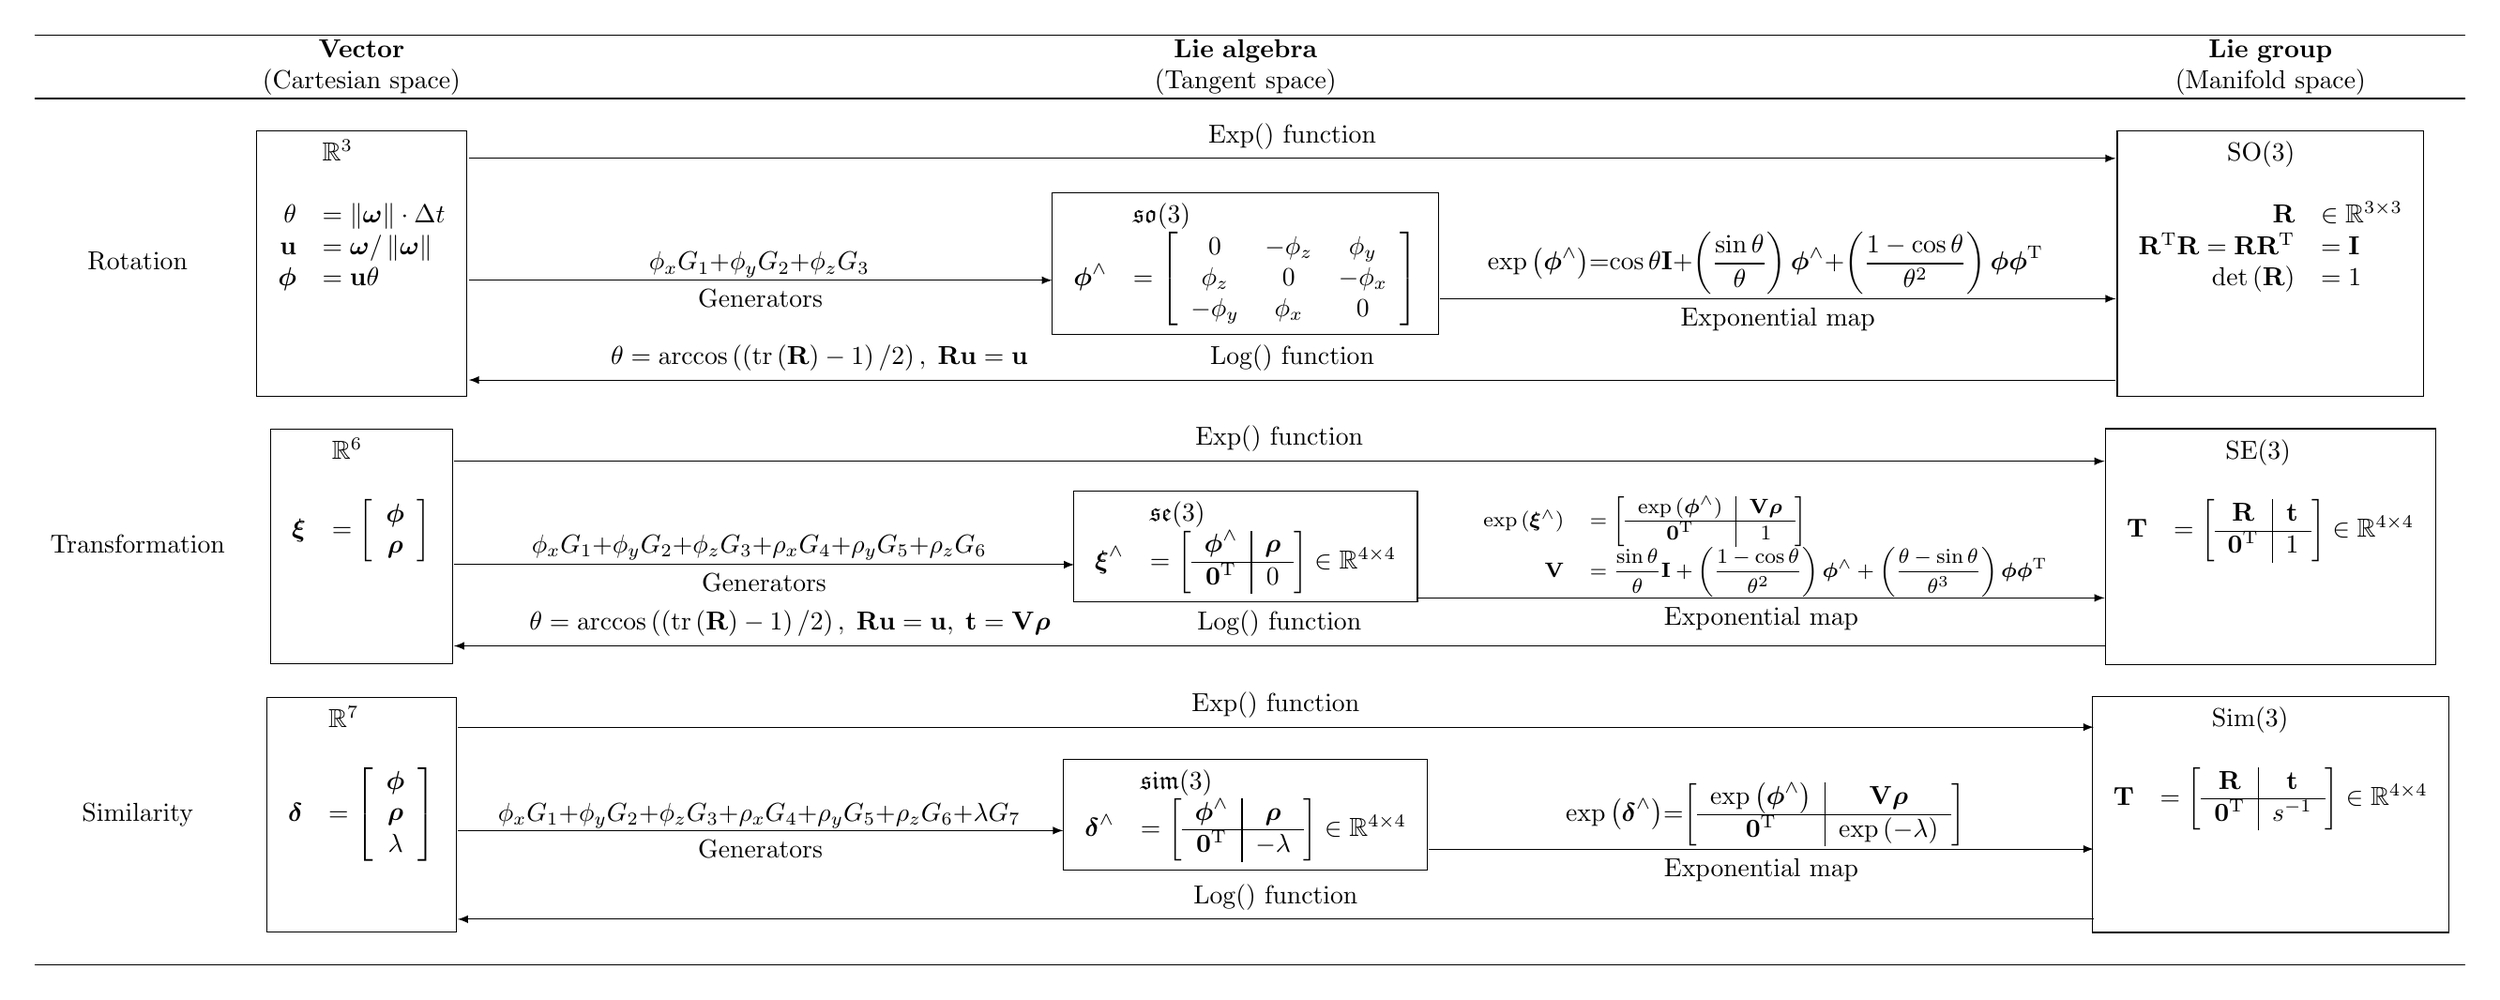
\begin{tikzpicture}[scale=1]

\node[below right] at (0.0,0.0) 
{$\begin{tabular}{cccccc}
\hline   &  \ensuremath{\mathbf{Vector}}  &   &  \ensuremath{\mathbf{Lie\ algebra}}  &  \ensuremath{}  & \ensuremath{\mathbf{Lie\ group}}\\
 & (Cartesian\ space) &  & (Tangent\ space) &  & (Manifold\ space)\\
\hline \text{} \\
  \ensuremath{\mathrm{Rotation}}  & \boxed{\begin{array}{rl}
 & \mathbb{R}^{3}\\
\\
\theta & =\left\Vert \boldsymbol{\omega}\right\Vert \cdot\Delta t\\
\mathbf{u} & =\boldsymbol{\omega}/\left\Vert \boldsymbol{\omega}\right\Vert \\
\boldsymbol{\phi} & =\mathbf{u}\theta\\
\\
\\
\\
\end{array}} & \ensuremath{\phi_{x}G_{1}}+\ensuremath{\phi_{y}G_{2}}+\ensuremath{\phi_{z}G_{3}} & \boxed{\begin{array}{rl}
 & \mathfrak{so}(3)\\
\boldsymbol{\phi}^{\wedge} & =\left[\begin{array}{ccc}
0 & -\phi_{z} & \phi_{y}\\
\phi_{z} & 0 & -\phi_{x}\\
-\phi_{y} & \phi_{x} & 0
\end{array}\right]
\end{array}} & \ensuremath{\exp\left(\boldsymbol{\phi}^{\wedge}\right)}=\ensuremath{\cos\theta}\ensuremath{\mathbf{I}}+\ensuremath{\left(\dfrac{\sin\theta}{\theta}\right)\boldsymbol{\phi}^{\wedge}}+\ensuremath{\left(\dfrac{1-\cos\theta}{\theta^{2}}\right)\boldsymbol{\phi}\boldsymbol{\phi}^{\mathrm{T}}} & \boxed{\begin{array}{rl}
\mathrm{SO}(3)\\
\\
\mathbf{R} & \in\mathbb{R}^{3\times3}\\
\mathbf{R}^{\mathrm{T}}\mathbf{R}=\mathbf{R}\mathbf{R}^{\mathrm{T}} & =\mathbf{I}\\
\det\left(\mathbf{R}\right) & =1\\
\\
\\
\\
\end{array}}\\
  \\
  \ensuremath{\mathrm{Transformation}}  & \boxed{\begin{array}{rl}
 & \mathbb{R}^{6}\\
\\
\boldsymbol{\xi} & =\left[\begin{array}{c}
\boldsymbol{\phi}\\
\boldsymbol{\rho}
\end{array}\right]\\
\\
\\
\\
\end{array}} & \ensuremath{\phi_{x}G_{1}}+\ensuremath{\phi_{y}G_{2}}+\ensuremath{\phi_{z}G_{3}}+\ensuremath{\rho_{x}G_{4}}+\ensuremath{\rho_{y}G_{5}}+\ensuremath{\rho_{z}G_{6}} & \boxed{\begin{array}{rl}
 & \mathfrak{se}(3)\\
\boldsymbol{\xi}^{\wedge} & =\left[\begin{array}{c|c}
\boldsymbol{\phi}^{\wedge} & \boldsymbol{\rho}\\
\hline \mathbf{0}^{\mathrm{T}} & 0
\end{array}\right]\in\mathbb{R}^{4\times4}
\end{array}} & \ensuremath{{\footnotesize \begin{array}{rl}
\exp\left(\boldsymbol{\xi}^{\wedge}\right) & =\left[\begin{array}{c|c}
\exp\left(\boldsymbol{\phi}^{\wedge}\right) & \mathbf{V}\boldsymbol{\rho}\\
\hline \mathbf{0}^{\mathrm{T}} & 1
\end{array}\right]\\
\mathbf{V} & =\dfrac{\sin\theta}{\theta}\mathbf{I}+\left(\dfrac{1-\cos\theta}{\theta^{2}}\right)\boldsymbol{\phi}^{\wedge}+\left(\dfrac{\theta-\sin\theta}{\theta^{3}}\right)\boldsymbol{\phi}\boldsymbol{\phi}^{\mathrm{T}}
\end{array}}} & \boxed{\begin{array}{rl}
 & \qquad\mathrm{SE}(3)\\
\\
\mathbf{T} & =\left[\begin{array}{c|c}
\mathbf{R} & \mathbf{t}\\
\hline \mathbf{0}^{\mathrm{T}} & 1
\end{array}\right]\in\mathbb{R}^{4\times4}\\
\\
\\
\\
\end{array}}\\
 \ensuremath{\mathrm{}} \\
Similarity  & \boxed{\begin{array}{rl}
 & \mathbb{R}^{7}\\
\\
\boldsymbol{\delta} & =\left[\begin{array}{c}
\boldsymbol{\phi}\\
\boldsymbol{\rho}\\
\lambda
\end{array}\right]\\
\\
\\
\end{array}} & \ensuremath{\phi_{x}G_{1}}+\ensuremath{\phi_{y}G_{2}}+\ensuremath{\phi_{z}G_{3}}+\ensuremath{\rho_{x}G_{4}}+\ensuremath{\rho_{y}G_{5}}+\ensuremath{\rho_{z}G_{6}}+\ensuremath{\lambda G_{7}} & \boxed{\begin{array}{rl}
 & \mathfrak{sim}(3)\\
\boldsymbol{\delta}^{\wedge} & =\left[\begin{array}{c|c}
\boldsymbol{\phi}^{\wedge} & \boldsymbol{\rho}\\
\hline \mathbf{0}^{\mathrm{T}} & -\lambda
\end{array}\right]\in\mathbb{R}^{4\times4}
\end{array}} & \ensuremath{\exp\left(\boldsymbol{\delta}^{\wedge}\right)}=\ensuremath{\left[\begin{array}{c|c}
\exp\left(\boldsymbol{\phi}^{\wedge}\right) & \mathbf{V}\boldsymbol{\rho}\\
\hline \mathbf{0}^{\mathrm{T}} & \exp\left(-\lambda\right)
\end{array}\right]} & \boxed{\begin{array}{rl}
 & \qquad\mathrm{Sim}(3)\\
\\
\mathbf{T} & =\left[\begin{array}{c|c}
\mathbf{R} & \mathbf{t}\\
\hline \mathbf{0}^{\mathrm{T}} & s^{-1}
\end{array}\right]\in\mathbb{R}^{4\times4}\\
\\
\\
\\
\end{array}}\\
\\
\hline \end{tabular}$};

\draw [->,>=latex] (6.0,-3.45) -- node [below] {Generators} (13.9,-3.45);
\draw [->,>=latex] (5.8,-7.30) -- node [below] {Generators} (14.2,-7.30);
\draw [->,>=latex] (5.85,-10.90) -- node [below] {Generators} (14.05,-10.90);

\draw [->,>=latex] (19.15,-3.70) -- node [below] {Exponential map} (28.30,-3.70);
\draw [->,>=latex] (18.85,-7.75) -- node [below] {Exponential map} (28.15,-7.75);
\draw [->,>=latex] (19.00,-11.15) -- node [below] {Exponential map} (28.00,-11.15);

\draw [->,>=latex] (6.0,-1.8) -- node [above] {Exp() function} (28.30,-1.8);
\draw [->,>=latex] (28.30,-4.8) -- node [above] {Log() function} (6.0,-4.8);
\node[above right] at (7.8,-4.8) {$\theta=\arccos\left(\left(\mathrm{tr}\left(\mathbf{R}\right)-1\right)/2\right),\;\mathbf{R}\mathbf{u}=\mathbf{u}$};

\draw [->,>=latex] (5.8,-5.9) -- node [above] {Exp() function} (28.15,-5.9);
\draw [->,>=latex] (28.15,-8.40) -- node [above] {Log() function} (5.8,-8.40);
\node[above right] at (6.7,-8.40) {$\theta=\arccos\left(\left(\mathrm{tr}\left(\mathbf{R}\right)-1\right)/2\right),\;\mathbf{R}\mathbf{u}=\mathbf{u},\;\mathbf{t}=\mathbf{V}\boldsymbol{\rho}$};

\draw [->,>=latex] (5.85,-9.5) -- node [above] {Exp() function} (28.00,-9.5);
\draw [->,>=latex] (28.00,-12.10) -- node [above] {Log() function} (5.85,-12.10);

\end{tikzpicture}

\end{document}

